% This is the Reed College LaTeX thesis template. Most of the work
% for the document class was done by Sam Noble (SN), as well as this
% template. Later comments etc. by Ben Salzberg (BTS). Additional
% restructuring and APA support by Jess Youngberg (JY).
% Your comments and suggestions are more than welcome; please email
% them to cus@reed.edu
%
% See https://www.reed.edu/cis/help/LaTeX/index.html for help. There are a
% great bunch of help pages there, with notes on
% getting started, bibtex, etc. Go there and read it if you're not
% already familiar with LaTeX.
%
% Any line that starts with a percent symbol is a comment.
% They won't show up in the document, and are useful for notes
% to yourself and explaining commands.
% Commenting also removes a line from the document;
% very handy for troubleshooting problems. -BTS

% As far as I know, this follows the requirements laid out in
% the 2002-2003 Senior Handbook. Ask a librarian to check the
% document before binding. -SN

%%
%% Preamble
%%
% \documentclass{<something>} must begin each LaTeX document
\documentclass[12pt,twoside]{reedthesis}
% Packages are extensions to the basic LaTeX functions. Whatever you
% want to typeset, there is probably a package out there for it.
% Chemistry (chemtex), screenplays, you name it.
% Check out CTAN to see: https://www.ctan.org/
%%
\usepackage{graphicx,latexsym}
\usepackage{amsmath}
\usepackage{amssymb,amsthm}
\usepackage{longtable,booktabs,setspace}
\usepackage{chemarr} %% Useful for one reaction arrow, useless if you're not a chem major
\usepackage[hyphens]{url}
% Added by CII
\usepackage{hyperref}
\usepackage{lmodern}
\usepackage{float}
\floatplacement{figure}{H}
% End of CII addition
\usepackage{rotating}

% Next line commented out by CII
%%% \usepackage{natbib}
% Comment out the natbib line above and uncomment the following two lines to use the new
% biblatex-chicago style, for Chicago A. Also make some changes at the end where the
% bibliography is included.
%\usepackage{biblatex-chicago}
%\bibliography{thesis}


% Added by CII (Thanks, Hadley!)
% Use ref for internal links
\renewcommand{\hyperref}[2][???]{\autoref{#1}}
\def\chapterautorefname{Chapter}
\def\sectionautorefname{Section}
\def\subsectionautorefname{Subsection}
% End of CII addition

% Added by CII
\usepackage{caption}
\captionsetup{width=5in}
% End of CII addition

% \usepackage{times} % other fonts are available like times, bookman, charter, palatino

% Syntax highlighting #22
  \usepackage{color}
  \usepackage{fancyvrb}
  \newcommand{\VerbBar}{|}
  \newcommand{\VERB}{\Verb[commandchars=\\\{\}]}
  \DefineVerbatimEnvironment{Highlighting}{Verbatim}{commandchars=\\\{\}}
  % Add ',fontsize=\small' for more characters per line
  \usepackage{framed}
  \definecolor{shadecolor}{RGB}{248,248,248}
  \newenvironment{Shaded}{\begin{snugshade}}{\end{snugshade}}
  \newcommand{\AlertTok}[1]{\textcolor[rgb]{0.94,0.16,0.16}{#1}}
  \newcommand{\AnnotationTok}[1]{\textcolor[rgb]{0.56,0.35,0.01}{\textbf{\textit{#1}}}}
  \newcommand{\AttributeTok}[1]{\textcolor[rgb]{0.77,0.63,0.00}{#1}}
  \newcommand{\BaseNTok}[1]{\textcolor[rgb]{0.00,0.00,0.81}{#1}}
  \newcommand{\BuiltInTok}[1]{#1}
  \newcommand{\CharTok}[1]{\textcolor[rgb]{0.31,0.60,0.02}{#1}}
  \newcommand{\CommentTok}[1]{\textcolor[rgb]{0.56,0.35,0.01}{\textit{#1}}}
  \newcommand{\CommentVarTok}[1]{\textcolor[rgb]{0.56,0.35,0.01}{\textbf{\textit{#1}}}}
  \newcommand{\ConstantTok}[1]{\textcolor[rgb]{0.00,0.00,0.00}{#1}}
  \newcommand{\ControlFlowTok}[1]{\textcolor[rgb]{0.13,0.29,0.53}{\textbf{#1}}}
  \newcommand{\DataTypeTok}[1]{\textcolor[rgb]{0.13,0.29,0.53}{#1}}
  \newcommand{\DecValTok}[1]{\textcolor[rgb]{0.00,0.00,0.81}{#1}}
  \newcommand{\DocumentationTok}[1]{\textcolor[rgb]{0.56,0.35,0.01}{\textbf{\textit{#1}}}}
  \newcommand{\ErrorTok}[1]{\textcolor[rgb]{0.64,0.00,0.00}{\textbf{#1}}}
  \newcommand{\ExtensionTok}[1]{#1}
  \newcommand{\FloatTok}[1]{\textcolor[rgb]{0.00,0.00,0.81}{#1}}
  \newcommand{\FunctionTok}[1]{\textcolor[rgb]{0.00,0.00,0.00}{#1}}
  \newcommand{\ImportTok}[1]{#1}
  \newcommand{\InformationTok}[1]{\textcolor[rgb]{0.56,0.35,0.01}{\textbf{\textit{#1}}}}
  \newcommand{\KeywordTok}[1]{\textcolor[rgb]{0.13,0.29,0.53}{\textbf{#1}}}
  \newcommand{\NormalTok}[1]{#1}
  \newcommand{\OperatorTok}[1]{\textcolor[rgb]{0.81,0.36,0.00}{\textbf{#1}}}
  \newcommand{\OtherTok}[1]{\textcolor[rgb]{0.56,0.35,0.01}{#1}}
  \newcommand{\PreprocessorTok}[1]{\textcolor[rgb]{0.56,0.35,0.01}{\textit{#1}}}
  \newcommand{\RegionMarkerTok}[1]{#1}
  \newcommand{\SpecialCharTok}[1]{\textcolor[rgb]{0.00,0.00,0.00}{#1}}
  \newcommand{\SpecialStringTok}[1]{\textcolor[rgb]{0.31,0.60,0.02}{#1}}
  \newcommand{\StringTok}[1]{\textcolor[rgb]{0.31,0.60,0.02}{#1}}
  \newcommand{\VariableTok}[1]{\textcolor[rgb]{0.00,0.00,0.00}{#1}}
  \newcommand{\VerbatimStringTok}[1]{\textcolor[rgb]{0.31,0.60,0.02}{#1}}
  \newcommand{\WarningTok}[1]{\textcolor[rgb]{0.56,0.35,0.01}{\textbf{\textit{#1}}}}

% To pass between YAML and LaTeX the dollar signs are added by CII
\title{Hierarchical Bayesian Modeling of Forest Attributes}
\author{Grayson White}
% The month and year that you submit your FINAL draft TO THE LIBRARY (May or December)
\date{May 2021}
\division{Mathematics and Natural Sciences}
\advisor{Kelly McConville}
\institution{Reed College}
\degree{Bachelor of Arts}
%If you have two advisors for some reason, you can use the following
% Uncommented out by CII
% End of CII addition

%%% Remember to use the correct department!
\department{Mathematics}
% if you're writing a thesis in an interdisciplinary major,
% uncomment the line below and change the text as appropriate.
% check the Senior Handbook if unsure.
%\thedivisionof{The Established Interdisciplinary Committee for}
% if you want the approval page to say "Approved for the Committee",
% uncomment the next line
%\approvedforthe{Committee}

% Added by CII
%%% Copied from knitr
%% maxwidth is the original width if it's less than linewidth
%% otherwise use linewidth (to make sure the graphics do not exceed the margin)
\makeatletter
\def\maxwidth{ %
  \ifdim\Gin@nat@width>\linewidth
    \linewidth
  \else
    \Gin@nat@width
  \fi
}
\makeatother

%Added by @MyKo101, code provided by @GerbrichFerdinands

\renewcommand{\contentsname}{Table of Contents}
% End of CII addition

\setlength{\parskip}{0pt}

% Added by CII

\providecommand{\tightlist}{%
  \setlength{\itemsep}{0pt}\setlength{\parskip}{0pt}}

\Acknowledgements{
I want to thank a few people.
}

\Dedication{
You can have a dedication here if you wish.
}

\Preface{
This is an example of a thesis setup to use the reed thesis document class
(for LaTeX) and the R bookdown package, in general.
}

\Abstract{
The preface pretty much says it all.

\par

Second paragraph of abstract starts here.
}

	\usepackage{amsmath}
\usepackage{booktabs}
\usepackage{caption}
\usepackage{longtable}
% End of CII addition
%%
%% End Preamble
%%
%
\begin{document}

% Everything below added by CII
  \maketitle

\frontmatter % this stuff will be roman-numbered
\pagestyle{empty} % this removes page numbers from the frontmatter
  \begin{acknowledgements}
    I want to thank a few people.
  \end{acknowledgements}
  \begin{preface}
    This is an example of a thesis setup to use the reed thesis document class
    (for LaTeX) and the R bookdown package, in general.
  \end{preface}
  \hypersetup{linkcolor=black}
  \setcounter{tocdepth}{2}
  \tableofcontents

  \listoftables

  \listoffigures
  \begin{abstract}
    The preface pretty much says it all.
    
    \par
    
    Second paragraph of abstract starts here.
  \end{abstract}
  \begin{dedication}
    You can have a dedication here if you wish.
  \end{dedication}
\mainmatter % here the regular arabic numbering starts
\pagestyle{fancyplain} % turns page numbering back on

\hypertarget{introduction}{%
\chapter*{Introduction}\label{introduction}}
\addcontentsline{toc}{chapter}{Introduction}

Welcome to the \emph{R Markdown} thesis template. This template is based on (and in many places copied directly from) the Reed College LaTeX template, but hopefully it will provide a nicer interface for those that have never used TeX or LaTeX before. Using \emph{R Markdown} will also allow you to easily keep track of your analyses in \textbf{R} chunks of code, with the resulting plots and output included as well. The hope is this \emph{R Markdown} template gets you in the habit of doing reproducible research, which benefits you long-term as a researcher, but also will greatly help anyone that is trying to reproduce or build onto your results down the road.

Hopefully, you won't have much of a learning period to go through and you will reap the benefits of a nicely formatted thesis. The use of LaTeX in combination with \emph{Markdown} is more consistent than the output of a word processor, much less prone to corruption or crashing, and the resulting file is smaller than a Word file. While you may have never had problems using Word in the past, your thesis is likely going to be about twice as large and complex as anything you've written before, taxing Word's capabilities. After working with \emph{Markdown} and \textbf{R} together for a few weeks, we are confident this will be your reporting style of choice going forward.

\textbf{Why use it?}

\emph{R Markdown} creates a simple and straightforward way to interface with the beauty of LaTeX. Packages have been written in \textbf{R} to work directly with LaTeX to produce nicely formatting tables and paragraphs. In addition to creating a user friendly interface to LaTeX, \emph{R Markdown} also allows you to read in your data, to analyze it and to visualize it using \textbf{R} functions, and also to provide the documentation and commentary on the results of your project. Further, it allows for \textbf{R} results to be passed inline to the commentary of your results. You'll see more on this later.

\textbf{Who should use it?}

Anyone who needs to use data analysis, math, tables, a lot of figures, complex cross-references, or who just cares about the final appearance of their document should use \emph{R Markdown}. Of particular use should be anyone in the sciences, but the user-friendly nature of \emph{Markdown} and its ability to keep track of and easily include figures, automatically generate a table of contents, index, references, table of figures, etc. should make it of great benefit to nearly anyone writing a thesis project.

\textbf{For additional help with bookdown}

Please visit \href{https://bookdown.org/yihui/bookdown/}{the free online bookdown reference guide}.

\hypertarget{rmd-basics}{%
\chapter{R Markdown Basics}\label{rmd-basics}}

Here is a brief introduction into using \emph{R Markdown}. \emph{Markdown} is a simple formatting syntax for authoring HTML, PDF, and MS Word documents. \emph{R Markdown} provides the flexibility of \emph{Markdown} with the implementation of \textbf{R} input and output. For more details on using \emph{R Markdown} see \url{https://rmarkdown.rstudio.com}.

Be careful with your spacing in \emph{Markdown} documents. While whitespace largely is ignored, it does at times give \emph{Markdown} signals as to how to proceed. As a habit, try to keep everything left aligned whenever possible, especially as you type a new paragraph. In other words, there is no need to indent basic text in the Rmd document (in fact, it might cause your text to do funny things if you do).

\hypertarget{lists}{%
\section{Lists}\label{lists}}

It's easy to create a list. It can be unordered like
\begin{itemize}
\tightlist
\item
  Item 1
\item
  Item 2
\end{itemize}
or it can be ordered like
\begin{enumerate}
\def\labelenumi{\arabic{enumi}.}
\tightlist
\item
  Item 1
\item
  Item 2
\end{enumerate}
Notice that I intentionally mislabeled Item 2 as number 4. \emph{Markdown} automatically figures this out! You can put any numbers in the list and it will create the list. Check it out below.

To create a sublist, just indent the values a bit (at least four spaces or a tab). (Here's one case where indentation is key!)
\begin{enumerate}
\def\labelenumi{\arabic{enumi}.}
\tightlist
\item
  Item 1
\item
  Item 2
\item
  Item 3
  \begin{itemize}
  \tightlist
  \item
    Item 3a
  \item
    Item 3b
  \end{itemize}
\end{enumerate}
\hypertarget{line-breaks}{%
\section{Line breaks}\label{line-breaks}}

Make sure to add white space between lines if you'd like to start a new paragraph. Look at what happens below in the outputted document if you don't:

Here is the first sentence. Here is another sentence. Here is the last sentence to end the paragraph.
This should be a new paragraph.

\emph{Now for the correct way:}

Here is the first sentence. Here is another sentence. Here is the last sentence to end the paragraph.

This should be a new paragraph.

\hypertarget{r-chunks}{%
\section{R chunks}\label{r-chunks}}

When you click the \textbf{Knit} button above a document will be generated that includes both content as well as the output of any embedded \textbf{R} code chunks within the document. You can embed an \textbf{R} code chunk like this (\texttt{cars} is a built-in \textbf{R} dataset):
\begin{Shaded}
\begin{Highlighting}[]
\KeywordTok{summary}\NormalTok{(cars)}
\end{Highlighting}
\end{Shaded}
\begin{verbatim}
     speed           dist       
 Min.   : 4.0   Min.   :  2.00  
 1st Qu.:12.0   1st Qu.: 26.00  
 Median :15.0   Median : 36.00  
 Mean   :15.4   Mean   : 42.98  
 3rd Qu.:19.0   3rd Qu.: 56.00  
 Max.   :25.0   Max.   :120.00  
\end{verbatim}
\hypertarget{inline-code}{%
\section{Inline code}\label{inline-code}}

If you'd like to put the results of your analysis directly into your discussion, add inline code like this:
\begin{quote}
The \texttt{cos} of \(2 \pi\) is 1.
\end{quote}
Another example would be the direct calculation of the standard deviation:
\begin{quote}
The standard deviation of \texttt{speed} in \texttt{cars} is 5.2876444.
\end{quote}
One last neat feature is the use of the \texttt{ifelse} conditional statement which can be used to output text depending on the result of an \textbf{R} calculation:
\begin{quote}
The standard deviation is less than 6.
\end{quote}
Note the use of \texttt{\textgreater{}} here, which signifies a quotation environment that will be indented.

As you see with \texttt{\$2\ \textbackslash{}pi\$} above, mathematics can be added by surrounding the mathematical text with dollar signs. More examples of this are in \protect\hyperlink{math-sci}{Mathematics and Science} if you uncomment the code in \protect\hyperlink{math}{Math}.

\hypertarget{including-plots}{%
\section{Including plots}\label{including-plots}}

You can also embed plots. For example, here is a way to use the base \textbf{R} graphics package to produce a plot using the built-in \texttt{pressure} dataset:

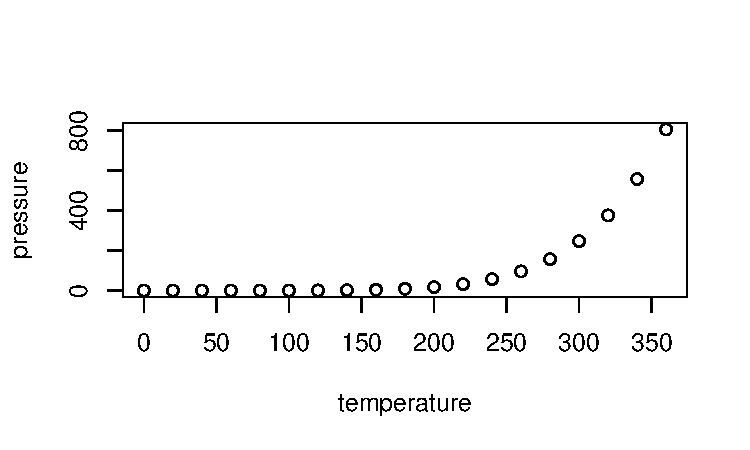
\includegraphics{thesis_files/figure-latex/pressure-1.pdf}

Note that the \texttt{echo=FALSE} parameter was added to the code chunk to prevent printing of the \textbf{R} code that generated the plot. There are plenty of other ways to add chunk options (like \texttt{fig.height} and \texttt{fig.width} in the chunk above). More information is available at \url{https://yihui.org/knitr/options/}.

Another useful chunk option is the setting of \texttt{cache=TRUE} as you see here. If document rendering becomes time consuming due to long computations or plots that are expensive to generate you can use knitr caching to improve performance. Later in this file, you'll see a way to reference plots created in \textbf{R} or external figures.

\hypertarget{loading-and-exploring-data}{%
\section{Loading and exploring data}\label{loading-and-exploring-data}}

Included in this template is a file called \texttt{flights.csv}. This file includes a subset of the larger dataset of information about all flights that departed from Seattle and Portland in 2014. More information about this dataset and its \textbf{R} package is available at \url{https://github.com/ismayc/pnwflights14}. This subset includes only Portland flights and only rows that were complete with no missing values. Merges were also done with the \texttt{airports} and \texttt{airlines} data sets in the \texttt{pnwflights14} package to get more descriptive airport and airline names.

We can load in this data set using the following commands:
\begin{Shaded}
\begin{Highlighting}[]
\CommentTok{# flights.csv is in the data directory}
\NormalTok{flights_path <-}\StringTok{ }\NormalTok{here}\OperatorTok{::}\KeywordTok{here}\NormalTok{(}\StringTok{"data"}\NormalTok{, }\StringTok{"flights.csv"}\NormalTok{)}
\CommentTok{# string columns will be read in as strings and not factors now}
\NormalTok{flights <-}\StringTok{ }\KeywordTok{read.csv}\NormalTok{(flights_path, }\DataTypeTok{stringsAsFactors =} \OtherTok{FALSE}\NormalTok{)}
\end{Highlighting}
\end{Shaded}
The data is now stored in the data frame called \texttt{flights} in \textbf{R}. To get a better feel for the variables included in this dataset we can use a variety of functions. Here we can see the dimensions (rows by columns) and also the names of the columns.
\begin{Shaded}
\begin{Highlighting}[]
\KeywordTok{dim}\NormalTok{(flights)}
\end{Highlighting}
\end{Shaded}
\begin{verbatim}
[1] 12649    16
\end{verbatim}
\begin{Shaded}
\begin{Highlighting}[]
\KeywordTok{names}\NormalTok{(flights)}
\end{Highlighting}
\end{Shaded}
\begin{verbatim}
 [1] "month"        "day"          "dep_time"     "dep_delay"   
 [5] "arr_time"     "arr_delay"    "carrier"      "tailnum"     
 [9] "flight"       "dest"         "air_time"     "distance"    
[13] "hour"         "minute"       "carrier_name" "dest_name"   
\end{verbatim}
Another good idea is to take a look at the dataset in table form. With this dataset having more than 20,000 rows, we won't explicitly show the results of the command here. I recommend you enter the command into the Console \textbf{\emph{after}} you have run the \textbf{R} chunks above to load the data into \textbf{R}.
\begin{Shaded}
\begin{Highlighting}[]
\KeywordTok{View}\NormalTok{(flights)}
\end{Highlighting}
\end{Shaded}
While not required, it is highly recommended you use the \texttt{dplyr} package to manipulate and summarize your data set as needed. It uses a syntax that is easy to understand using chaining operations. Below I've created a few examples of using \texttt{dplyr} to get information about the Portland flights in 2014. You will also see the use of the \texttt{ggplot2} package, which produces beautiful, high-quality academic visuals.

We begin by checking to ensure that needed packages are installed and then we load them into our current working environment:
\begin{Shaded}
\begin{Highlighting}[]
\CommentTok{# List of packages required for this analysis}
\NormalTok{pkg <-}\StringTok{ }\KeywordTok{c}\NormalTok{(}\StringTok{"dplyr"}\NormalTok{, }\StringTok{"ggplot2"}\NormalTok{, }\StringTok{"knitr"}\NormalTok{, }\StringTok{"bookdown"}\NormalTok{)}
\CommentTok{# Check if packages are not installed and assign the}
\CommentTok{# names of the packages not installed to the variable new.pkg}
\NormalTok{new.pkg <-}\StringTok{ }\NormalTok{pkg[}\OperatorTok{!}\NormalTok{(pkg }\OperatorTok\StringTok{ }\KeywordTok{installed.packages}\NormalTok{())]}
\CommentTok{# If there are any packages in the list that aren't installed,}
\CommentTok{# install them}
\ControlFlowTok{if}\NormalTok{ (}\KeywordTok{length}\NormalTok{(new.pkg)) \{}
  \KeywordTok{install.packages}\NormalTok{(new.pkg, }\DataTypeTok{repos =} \StringTok{"https://cran.rstudio.com"}\NormalTok{)}
\NormalTok{\}}
\CommentTok{# Load packages}
\KeywordTok{library}\NormalTok{(thesisdown)}
\KeywordTok{library}\NormalTok{(dplyr)}
\KeywordTok{library}\NormalTok{(ggplot2)}
\KeywordTok{library}\NormalTok{(knitr)}
\end{Highlighting}
\end{Shaded}
\clearpage

The example we show here does the following:
\begin{itemize}
\item
  Selects only the \texttt{carrier\_name} and \texttt{arr\_delay} from the \texttt{flights} dataset and then assigns this subset to a new variable called \texttt{flights2}.
\item
  Using \texttt{flights2}, we determine the largest arrival delay for each of the carriers.
\end{itemize}
\begin{Shaded}
\begin{Highlighting}[]
\NormalTok{flights2 <-}\StringTok{ }\NormalTok{flights }\OperatorTok
\StringTok{  }\KeywordTok{select}\NormalTok{(carrier_name, arr_delay)}
\NormalTok{max_delays <-}\StringTok{ }\NormalTok{flights2 }\OperatorTok
\StringTok{  }\KeywordTok{group_by}\NormalTok{(carrier_name) }\OperatorTok
\StringTok{  }\KeywordTok{summarize}\NormalTok{(}\DataTypeTok{max_arr_delay =} \KeywordTok{max}\NormalTok{(arr_delay, }\DataTypeTok{na.rm =} \OtherTok{TRUE}\NormalTok{))}
\end{Highlighting}
\end{Shaded}
\begin{verbatim}
`summarise()` ungrouping output (override with `.groups` argument)
\end{verbatim}
A useful function in the \texttt{knitr} package for making nice tables in \emph{R Markdown} is called \texttt{kable}. It is much easier to use than manually entering values into a table by copying and pasting values into Excel or LaTeX. This again goes to show how nice reproducible documents can be! (Note the use of \texttt{results="asis"}, which will produce the table instead of the code to create the table.) The \texttt{caption.short} argument is used to include a shorter title to appear in the List of Tables.
\begin{Shaded}
\begin{Highlighting}[]
\KeywordTok{kable}\NormalTok{(max_delays,}
  \DataTypeTok{col.names =} \KeywordTok{c}\NormalTok{(}\StringTok{"Airline"}\NormalTok{, }\StringTok{"Max Arrival Delay"}\NormalTok{),}
  \DataTypeTok{caption =} \StringTok{"Maximum Delays by Airline"}\NormalTok{,}
  \DataTypeTok{caption.short =} \StringTok{"Max Delays by Airline"}\NormalTok{,}
  \DataTypeTok{longtable =} \OtherTok{TRUE}\NormalTok{,}
  \DataTypeTok{booktabs =} \OtherTok{TRUE}
\NormalTok{)}
\end{Highlighting}
\end{Shaded}
\begin{longtable}[t]{lr}
\caption[Max Delays by Airline]{\label{tab:maxdelays}Maximum Delays by Airline}\\
\toprule
Airline & Max Arrival Delay\\
\midrule
Alaska Airlines Inc. & 338\\
American Airlines Inc. & 1539\\
Delta Air Lines Inc. & 371\\
Frontier Airlines Inc. & 166\\
Hawaiian Airlines Inc. & 116\\
\addlinespace
JetBlue Airways & 256\\
SkyWest Airlines Inc. & 321\\
Southwest Airlines Co. & 315\\
United Air Lines Inc. & 319\\
US Airways Inc. & 347\\
\addlinespace
Virgin America & 366\\
\bottomrule
\end{longtable}
The last two options make the table a little easier-to-read.

We can further look into the properties of the largest value here for American Airlines Inc.~To do so, we can isolate the row corresponding to the arrival delay of 1539 minutes for American in our original \texttt{flights} dataset.
\begin{Shaded}
\begin{Highlighting}[]
\NormalTok{flights }\OperatorTok
\StringTok{  }\KeywordTok{filter}\NormalTok{(}
\NormalTok{    arr_delay }\OperatorTok{==}\StringTok{ }\DecValTok{1539}\NormalTok{,}
\NormalTok{    carrier_name }\OperatorTok{==}\StringTok{ "American Airlines Inc."}
\NormalTok{  ) }\OperatorTok
\StringTok{  }\KeywordTok{select}\NormalTok{(}\OperatorTok{-}\KeywordTok{c}\NormalTok{(}
\NormalTok{    month, day, carrier, dest_name, hour,}
\NormalTok{    minute, carrier_name, arr_delay}
\NormalTok{  ))}
\end{Highlighting}
\end{Shaded}
\begin{verbatim}
  dep_time dep_delay arr_time tailnum flight dest air_time distance
1     1403      1553     1934  N595AA   1568  DFW      182     1616
\end{verbatim}
We see that the flight occurred on March 3rd and departed a little after 2 PM on its way to Dallas/Fort Worth. Lastly, we show how we can visualize the arrival delay of all departing flights from Portland on March 3rd against time of departure.
\begin{Shaded}
\begin{Highlighting}[]
\NormalTok{flights }\OperatorTok
\StringTok{  }\KeywordTok{filter}\NormalTok{(month }\OperatorTok{==}\StringTok{ }\DecValTok{3}\NormalTok{, day }\OperatorTok{==}\StringTok{ }\DecValTok{3}\NormalTok{) }\OperatorTok
\StringTok{  }\KeywordTok{ggplot}\NormalTok{(}\KeywordTok{aes}\NormalTok{(}\DataTypeTok{x =}\NormalTok{ dep_time, }\DataTypeTok{y =}\NormalTok{ arr_delay)) }\OperatorTok{+}
\StringTok{  }\KeywordTok{geom_point}\NormalTok{()}
\end{Highlighting}
\end{Shaded}
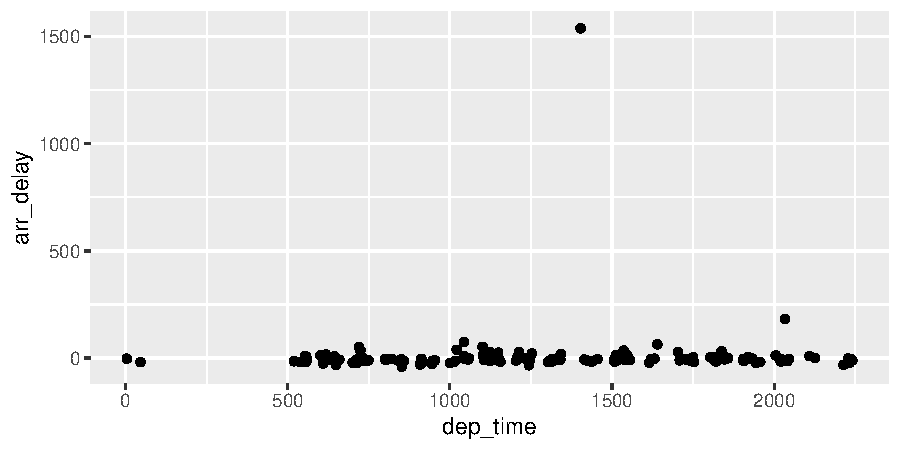
\includegraphics{thesis_files/figure-latex/march3plot-1.pdf}

\hypertarget{additional-resources}{%
\section{Additional resources}\label{additional-resources}}
\begin{itemize}
\item
  \emph{Markdown} Cheatsheet - \url{https://github.com/adam-p/markdown-here/wiki/Markdown-Cheatsheet}
\item
  \emph{R Markdown}
  \begin{itemize}
  \tightlist
  \item
    Reference Guide - \url{https://www.rstudio.com/wp-content/uploads/2015/03/rmarkdown-reference.pdf}
  \item
    Cheatsheet - \url{https://github.com/rstudio/cheatsheets/raw/master/rmarkdown-2.0.pdf}
  \end{itemize}
\item
  \emph{RStudio IDE}
  \begin{itemize}
  \tightlist
  \item
    Cheatsheet - \url{https://github.com/rstudio/cheatsheets/raw/master/rstudio-ide.pdf}
  \item
    Official website - \url{https://rstudio.com/products/rstudio/}
  \end{itemize}
\item
  Introduction to \texttt{dplyr} - \url{https://cran.rstudio.com/web/packages/dplyr/vignettes/dplyr.html}
\item
  \texttt{ggplot2}
  \begin{itemize}
  \tightlist
  \item
    Documentation - \url{https://ggplot2.tidyverse.org/}
  \item
    Cheatsheet - \url{https://github.com/rstudio/cheatsheets/raw/master/data-visualization-2.1.pdf}
  \end{itemize}
\end{itemize}
\hypertarget{math-sci}{%
\chapter{Mathematics and Science}\label{math-sci}}

\hypertarget{math}{%
\section{Math}\label{math}}

\TeX~is the best way to typeset mathematics. Donald Knuth designed \TeX~when he got frustrated at how long it was taking the typesetters to finish his book, which contained a lot of mathematics. One nice feature of \emph{R Markdown} is its ability to read LaTeX code directly.

If you are doing a thesis that will involve lots of math, you will want to read the following section which has been commented out. If you're not going to use math, skip over or delete this next commented section.

\hypertarget{chemistry-101-symbols}{%
\section{Chemistry 101: Symbols}\label{chemistry-101-symbols}}

Chemical formulas will look best if they are not italicized. Get around math mode's automatic italicizing in LaTeX by using the argument \texttt{\$\textbackslash{}mathrm\{formula\ here\}\$}, with your formula inside the curly brackets. (Notice the use of the backticks here which enclose text that acts as code.)

So, \(\mathrm{Fe_2^{2+}Cr_2O_4}\) is written \texttt{\$\textbackslash{}mathrm\{Fe\_2\^{}\{2+\}Cr\_2O\_4\}\$}.

\noindent Exponent or Superscript: \(\mathrm{O^-}\)

\noindent Subscript: \(\mathrm{CH_4}\)

To stack numbers or letters as in \(\mathrm{Fe_2^{2+}}\), the subscript is defined first, and then the superscript is defined.

\noindent Bullet: CuCl \(\bullet\) \(\mathrm{7H_{2}O}\)

\noindent Delta: \(\Delta\)

\noindent Reaction Arrows: \(\longrightarrow\) or \(\xrightarrow{solution}\)

\noindent Resonance Arrows: \(\leftrightarrow\)

\noindent Reversible Reaction Arrows: \(\rightleftharpoons\)

\hypertarget{typesetting-reactions}{%
\subsection{Typesetting reactions}\label{typesetting-reactions}}

You may wish to put your reaction in an equation environment, which means that LaTeX will place the reaction where it fits and will number the equations for you.
\begin{equation}
  \mathrm{C_6H_{12}O_6  + 6O_2} \longrightarrow \mathrm{6CO_2 + 6H_2O}
  \label{eq:reaction}
\end{equation}
We can reference this combustion of glucose reaction via Equation \eqref{eq:reaction}.

\hypertarget{other-examples-of-reactions}{%
\subsection{Other examples of reactions}\label{other-examples-of-reactions}}

\(\mathrm{NH_4Cl_{(s)}}\) \(\rightleftharpoons\) \(\mathrm{NH_{3(g)}+HCl_{(g)}}\)

\noindent \(\mathrm{MeCH_2Br + Mg}\) \(\xrightarrow[below]{above}\) \(\mathrm{MeCH_2\bullet Mg \bullet Br}\)

\hypertarget{physics}{%
\section{Physics}\label{physics}}

Many of the symbols you will need can be found on the math page \url{https://web.reed.edu/cis/help/latex/math.html} and the Comprehensive LaTeX Symbol Guide (\url{https://mirror.utexas.edu/ctan/info/symbols/comprehensive/symbols-letter.pdf}).

\hypertarget{biology}{%
\section{Biology}\label{biology}}

You will probably find the resources at \url{https://www.lecb.ncifcrf.gov/~toms/latex.html} helpful, particularly the links to bsts for various journals. You may also be interested in TeXShade for nucleotide typesetting (\url{https://homepages.uni-tuebingen.de/beitz/txe.html}). Be sure to read the proceeding chapter on graphics and tables.

\hypertarget{data}{%
\chapter{Data}\label{data}}

\hypertarget{the-forest-inventory-analysis-program}{%
\section{The Forest Inventory \& Analysis Program}\label{the-forest-inventory-analysis-program}}

The Forest Inventory \& Analysis Program (FIA) is a program within the United States Forest Service which aims to collect information and data in order to assess the country's forests. The FIA has been continuously operating since 1930 and their official mission is to ``make and keep current a comprehensive inventory and analysis of the present and prospective conditions of and requirements for the renewable resources of the forest and rangelands of the US.'' (Source: \url{https://www.fia.fs.fed.us/about/about_us/}).

The FIA collects data all throughout the United States by completing a survey each year of many plots of land. The units measured by the FIA and their ground crews are approximately 30 m by 30 m hexagonal units. Due to the vast size of the United States and immense amount of forested land, it would be nearly impossible for the FIA to attain population data for the country, so they use sampling instead. The FIA samples from the population of 30 m by 30 m hexagonal units by using a geographically-based systematic sampling design (Source: McConville et al, 2020). The FIA chooses these samples by first overlaying a hexagonal grid over the United States where each hexagon contains approximately 6000 acres of land. Then, they fill these hexagons with much smaller hexagons and randomly sample from the population of small hexagons. Then, ground crews go to these sampled small hexagons and collect variables such as basal area, trees per acre, etc. This plot level data is what we are working with throughout the duration of the thesis.

\hypertarget{the-interior-west}{%
\section{The Interior West}\label{the-interior-west}}

While the FIA collects data in all regions of the United States, the analyses done in this thesis uses data from the Interior West Forest Inventory and Analysis Unit (IW-FIA). Data from this unit will henceforth be refered to as data from ``the Interior West''. The Interior West is defined as a broad region of the United States, covering the states of Arizona, Colorado, Idaho, Montana, Nevada, New Mexico, Utah, and Wyoming. For reference we have provided the Interior West colored green on a map of the continental United States:
\begin{center}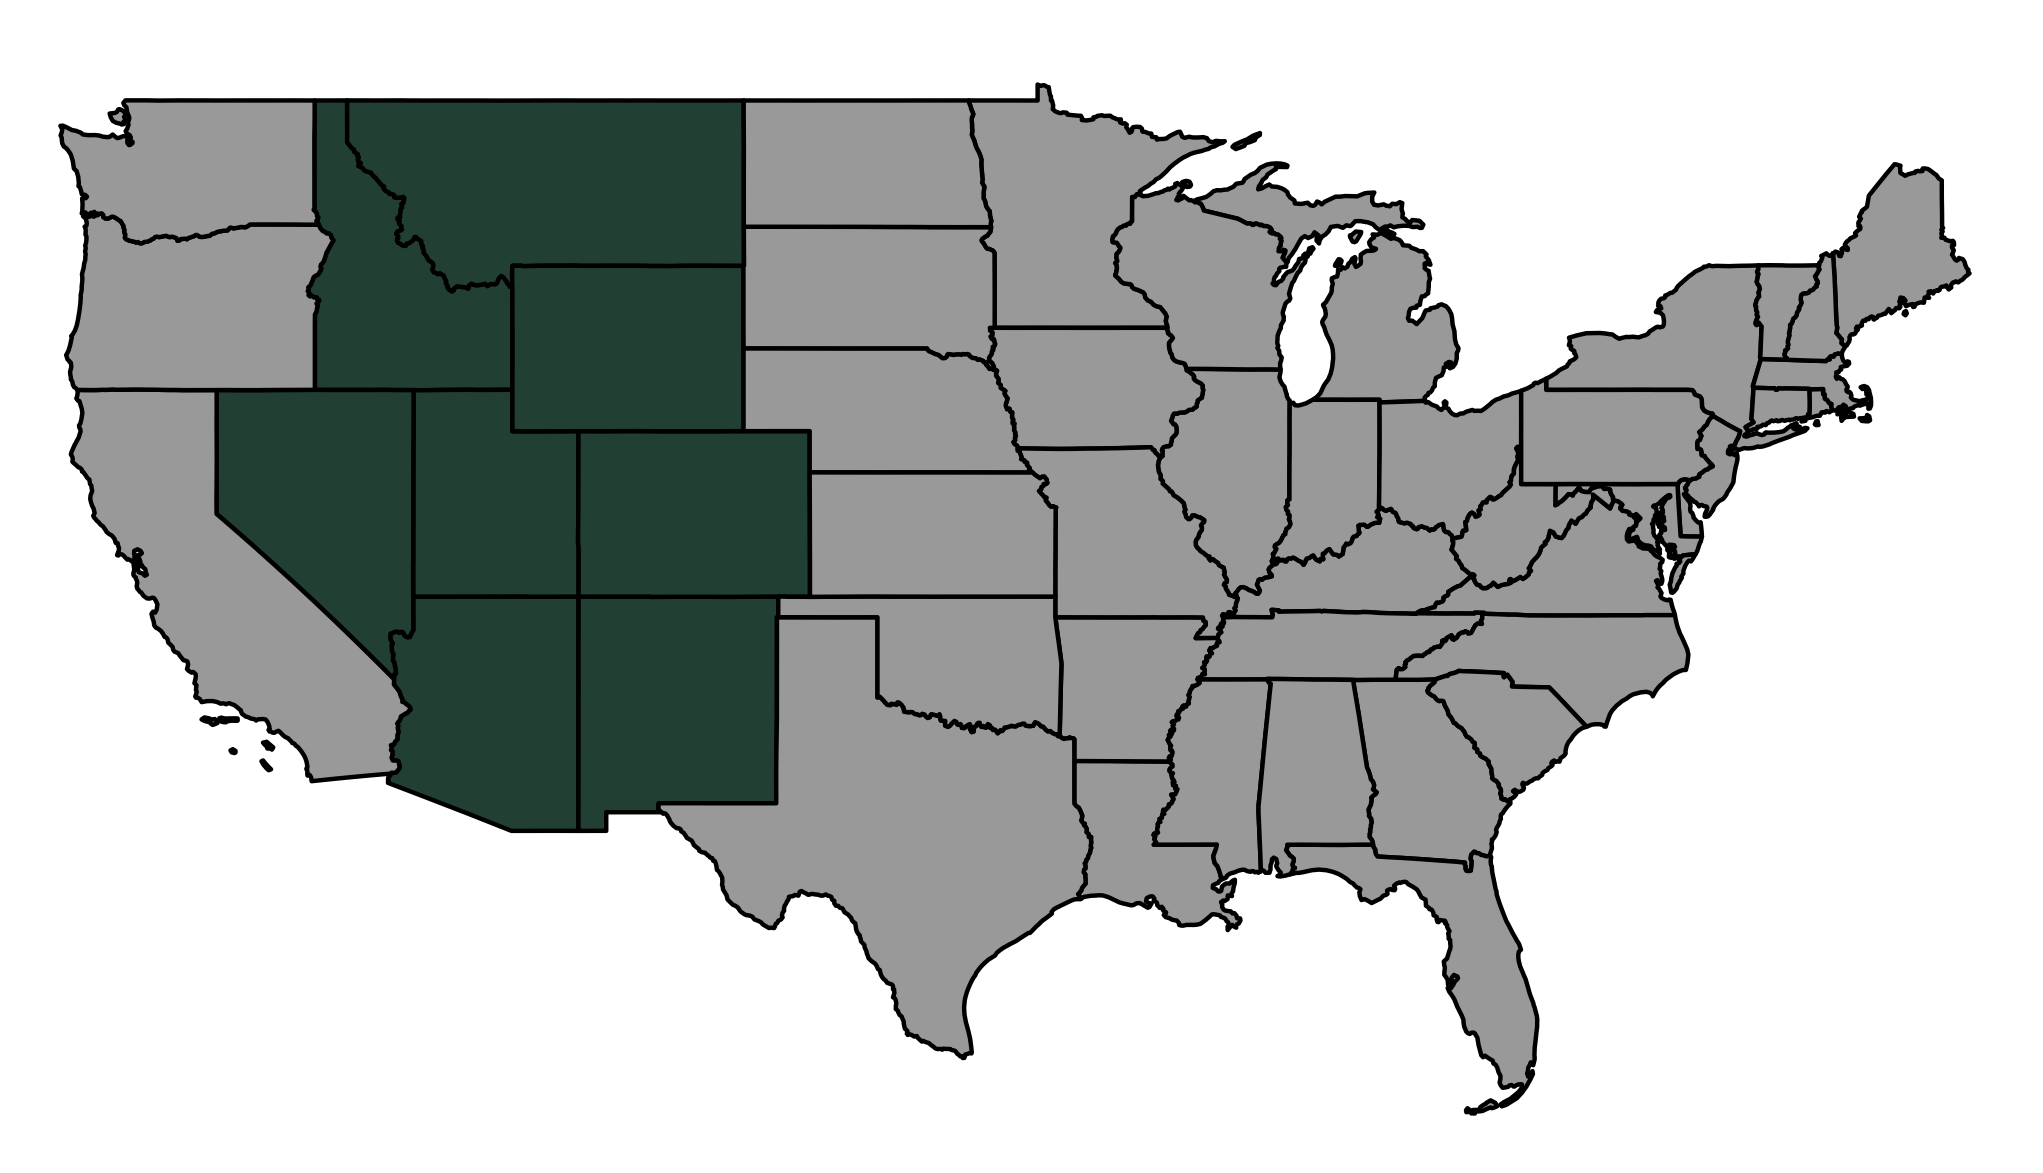
\includegraphics[width=29.17in]{figure/interior-west-on-usa} \end{center}

The IW-FIA collects annual inventories of the Interior West, with the goal of covering 10\% of the region each year, so every decade the IW-FIA should have measurement of 100\% of each Interior West state's forests.

The Interior West region itself contains the states which encompass the Rocky Mountains along with some other smaller mountain ranges. The Interior West contains 855,767 square miles of land which has an extremely diverse landscape ranging from the high mountain peaks of the Rockies to flat desert plains in Nevada and other Interior West states. Along with desert and mountains, the Interior West also includes parts of the Great Plains.

\hypertarget{our-data-specifics}{%
\section{Our Data: Specifics}\label{our-data-specifics}}

The data used in this thesis was collected by the Forest Inventory and Analysis Program (FIA) in the span of 10 years from 2007 to 2017. While this data was collected over this 10 year period, the analyses done throughout this thesis are under the assumption that this is a ``snapshot'' of the Interior West at some moment in time. Thus we do not consider any temporal features of this dataset, however the inventory year information is available to us. The data we have is plot-level data for the Interior West region of the United States, where the data for each plot is collected by FIA and its crew members.

The dataframe used in this thesis is a joined dataframe derived from two FIA datasets of the Interior West, \texttt{spatial} and \texttt{response}. The \texttt{spatial} dataframe contains 89444 observations and 70 variables, most notably two remotely sensed predictor variables (\texttt{forprob} and \texttt{forbio}), location information, and ecosubsection. The \texttt{response} dataframe contains 86085 observations and 67 variables, most notably four predictor variables collected by FIA crew members (\texttt{BALIVE\_TPA}, \texttt{CNTLIVE\_TPA}, \texttt{BIOLIVE\_TPA}, and \texttt{VOLNLIVE\_TPA}), location information, and ecosubsection. We join these dataframes by their unique plot number, and subset the number of variables significantly to 19 variables which contain plot information, longitude \& lattitude, elevation, predictor variables, response variables, ecosubsection, ecosection, and province. The resulting joined dataframe has 86085 rows as these are the rows which share the same plots between the \texttt{response} and \texttt{spatial} dataframes. We can see the first few rows of the dataframe with relevant columns selected:

\captionsetup[table]{labelformat=empty,skip=1pt}
\begin{longtable}{rrrrrrrrr}
\toprule
PLOT & LON & LAT & ELEV & forgrp & forprob & demLF & forbio & BALIVE\_TPA \\ 
\midrule
83657 & -111.3261 & 35.02106 & 6680 & 180 & 1 & 2080 & 12.67684 & 236.1169 \\ 
87963 & -109.9398 & 36.59399 & 5550 & 0 & 0 & 1700 & 0.00000 & 0.0000 \\ 
84186 & -109.9925 & 36.27860 & 7510 & 180 & 1 & 2305 & 10.57715 & 105.3212 \\ 
87499 & -109.9058 & 35.32838 & 5630 & 0 & 0 & 1717 & 0.00000 & 0.0000 \\ 
88091 & -109.9024 & 34.83752 & 5510 & 0 & 0 & 1672 & 0.00000 & 0.0000 \\ 
80842 & -109.9774 & 33.52990 & 5920 & 180 & 1 & 1828 & 14.46534 & 149.7189 \\ 
\bottomrule
\end{longtable}
\captionsetup[table]{labelformat=empty,skip=1pt}
\begin{longtable}{rrrlll}
\toprule
CNTLIVE\_TPA & BIOLIVE\_TPA & VOLNLIVE\_TPA & subsection & section & province \\ 
\midrule
555.3678 & 43.08024 & 2066.3352 & M313Ak & M313A & M313 \\ 
0.0000 & 0.00000 & 0.0000 & 313Ac & 313A & 313 \\ 
108.3248 & 18.02096 & 988.9084 & 313Ap & 313A & 313 \\ 
0.0000 & 0.00000 & 0.0000 & 313Db & 313D & 313 \\ 
0.0000 & 0.00000 & 0.0000 & 313Db & 313D & 313 \\ 
273.5608 & 21.76656 & 1381.8511 & 313Cd & 313C & 313 \\ 
\bottomrule
\end{longtable}
While the data covers the Interior West as a whole, we have very granular information, as each row represents a plot sampled by the FIA. The data also includes variables that subset the Interior West into provinces which contain ecosections, and these ecosections contain ecosubsections. In our data, on average, each ecosection contains approximately 7.06 ecosubsections, and each province contains an average of 4.86 ecosections. So, an average province then contains just over 34 ecosubsections. The data we have covers a total of 14 provinces, 68 ecosections, and 480 ecosubsections. The hierarchical struture of the data and nestedness of the ecosubsections within ecosections within provinces lends itself to be able to create hierarchical models which borrow strength from surrounding areas.

While this data contains a multitude of variables, the analyses done in this thesis focus on four key response variables and two explanatory variables. The response variables used are basal area (square-foot), trees per acre, above-ground biomass (lbs), and net volume (ft\^{}3). These variables are coded as \texttt{BALIVE\_TPA}, \texttt{CNTLIVE\_TPA}, \texttt{BIOLIVE\_TPA}, and \texttt{VOLNLIVE\_TPA}, respectively. We can look at the average of these variables across the Interior West region by ecosubsection in the four following maps of the interior west.
\begin{center}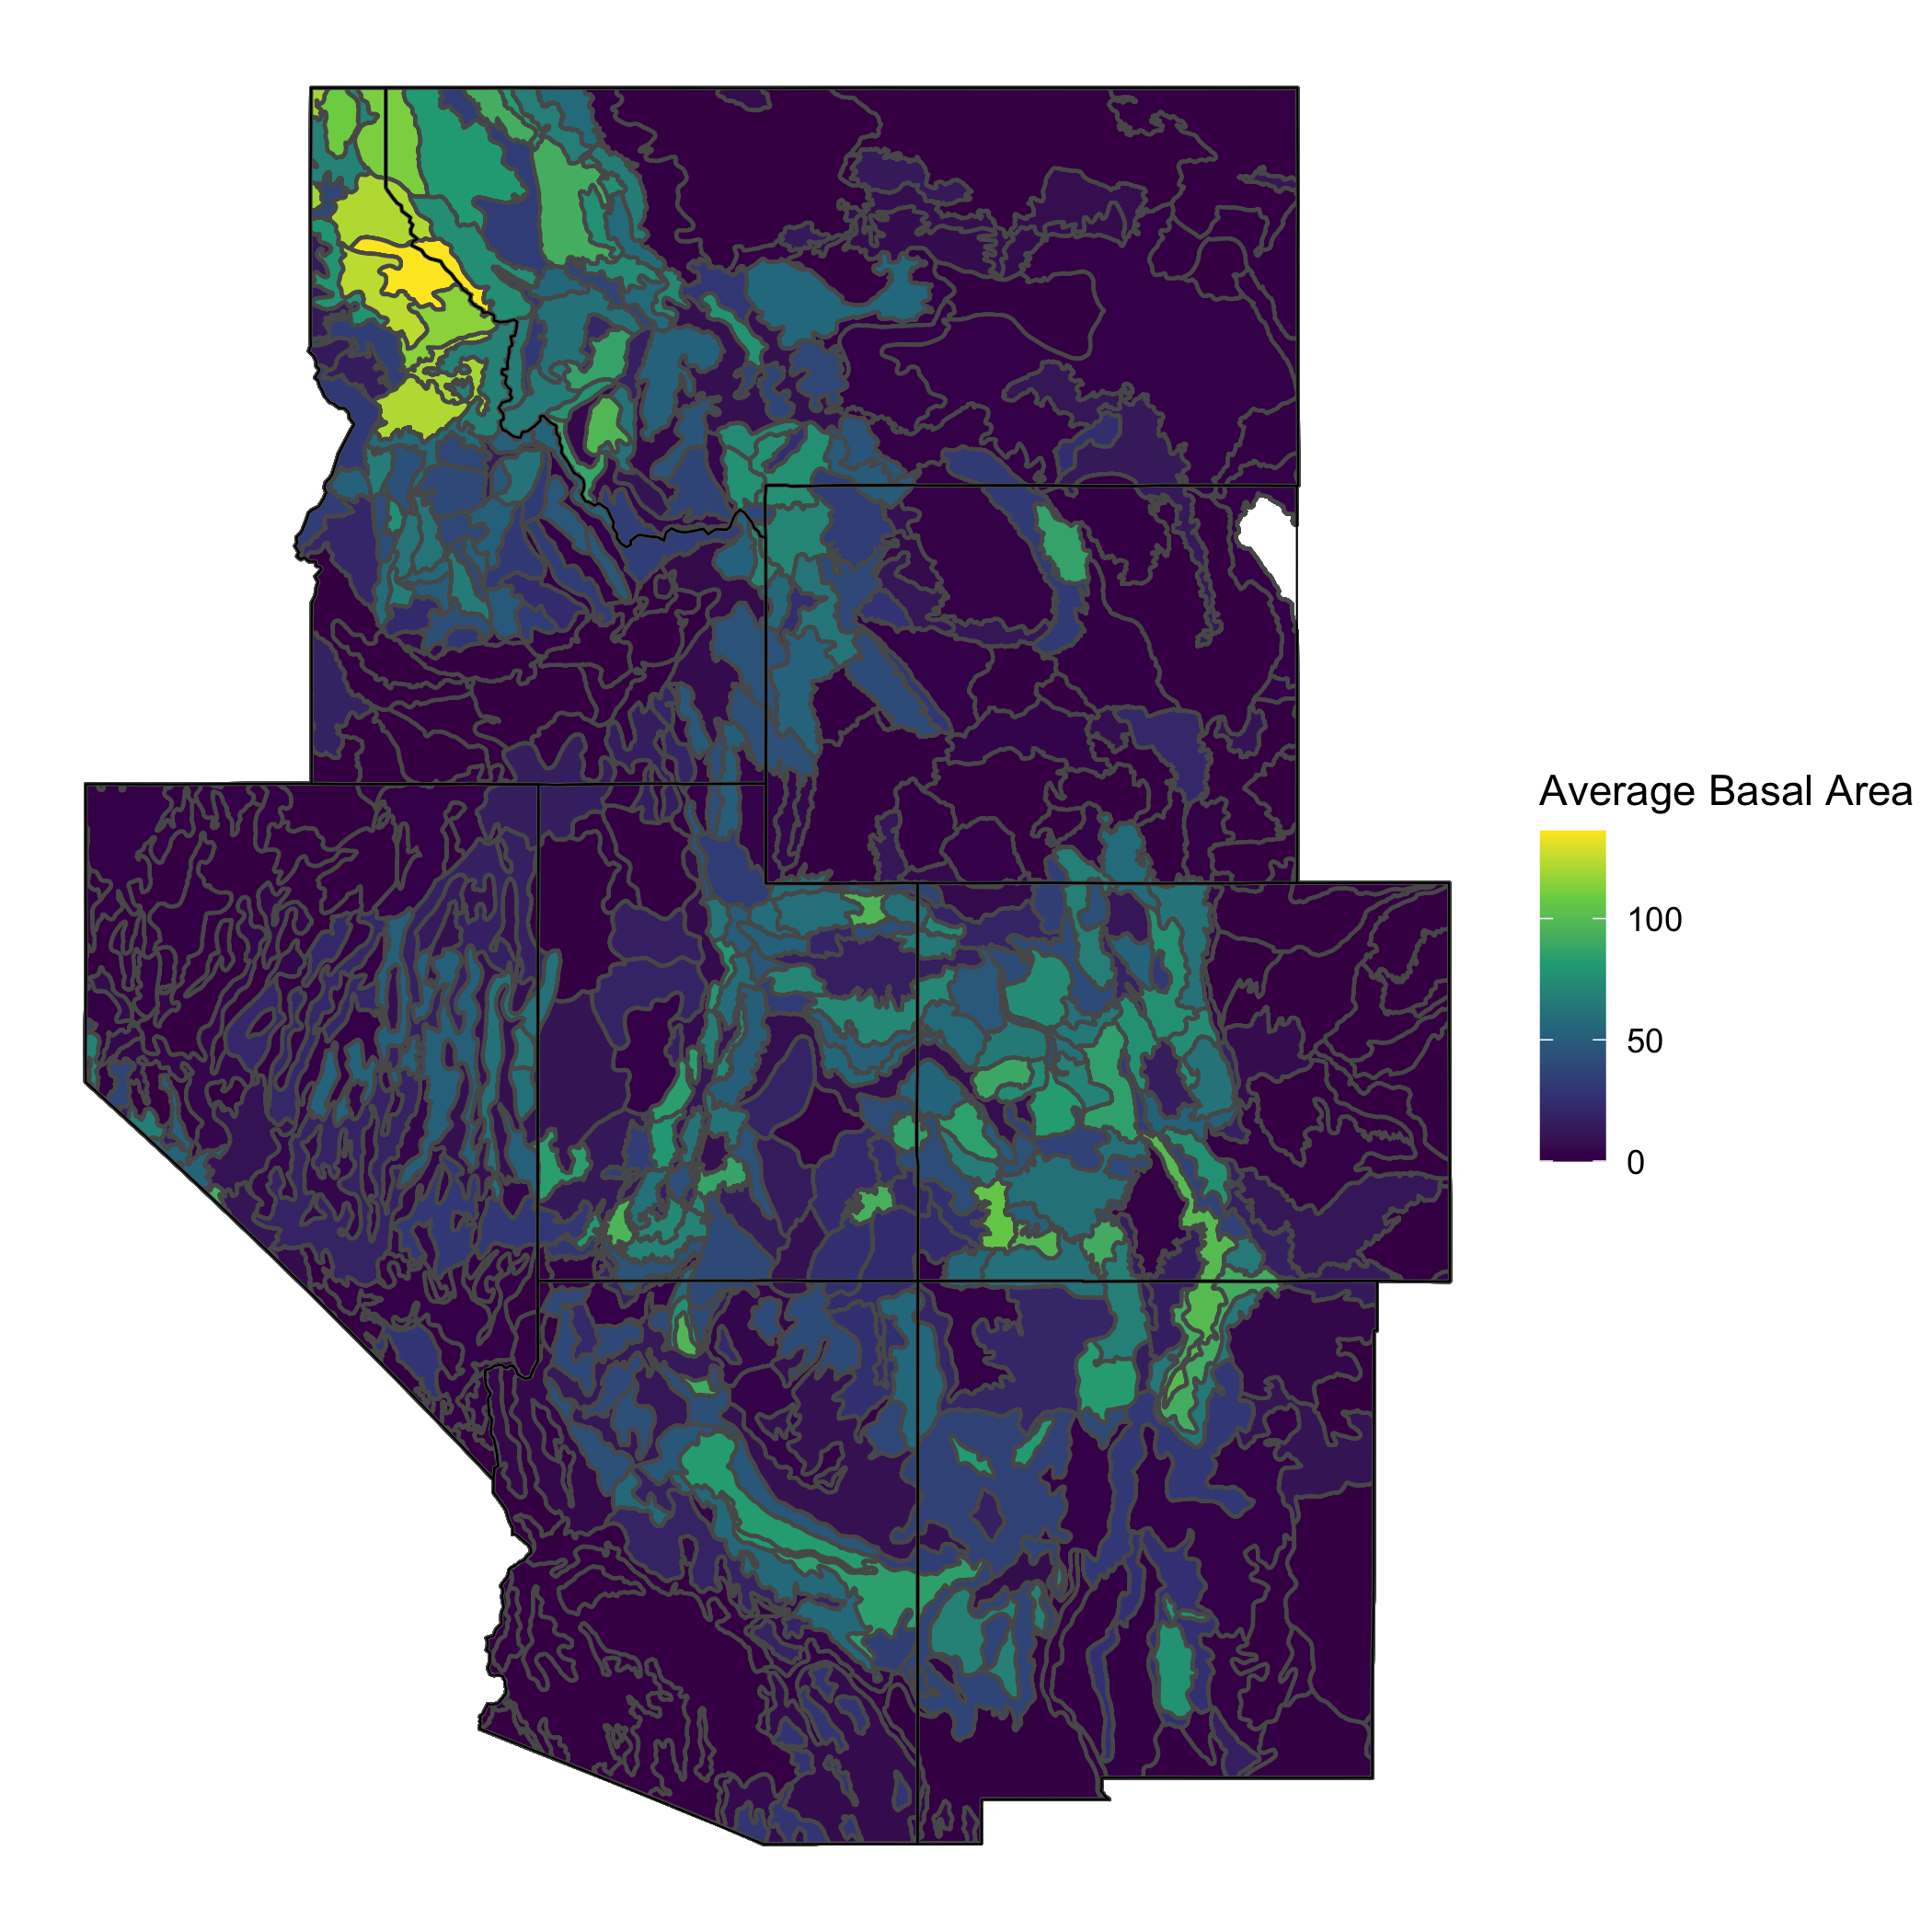
\includegraphics[width=0.65\linewidth,height=0.65\textheight]{figure/basal} \end{center}
\begin{center}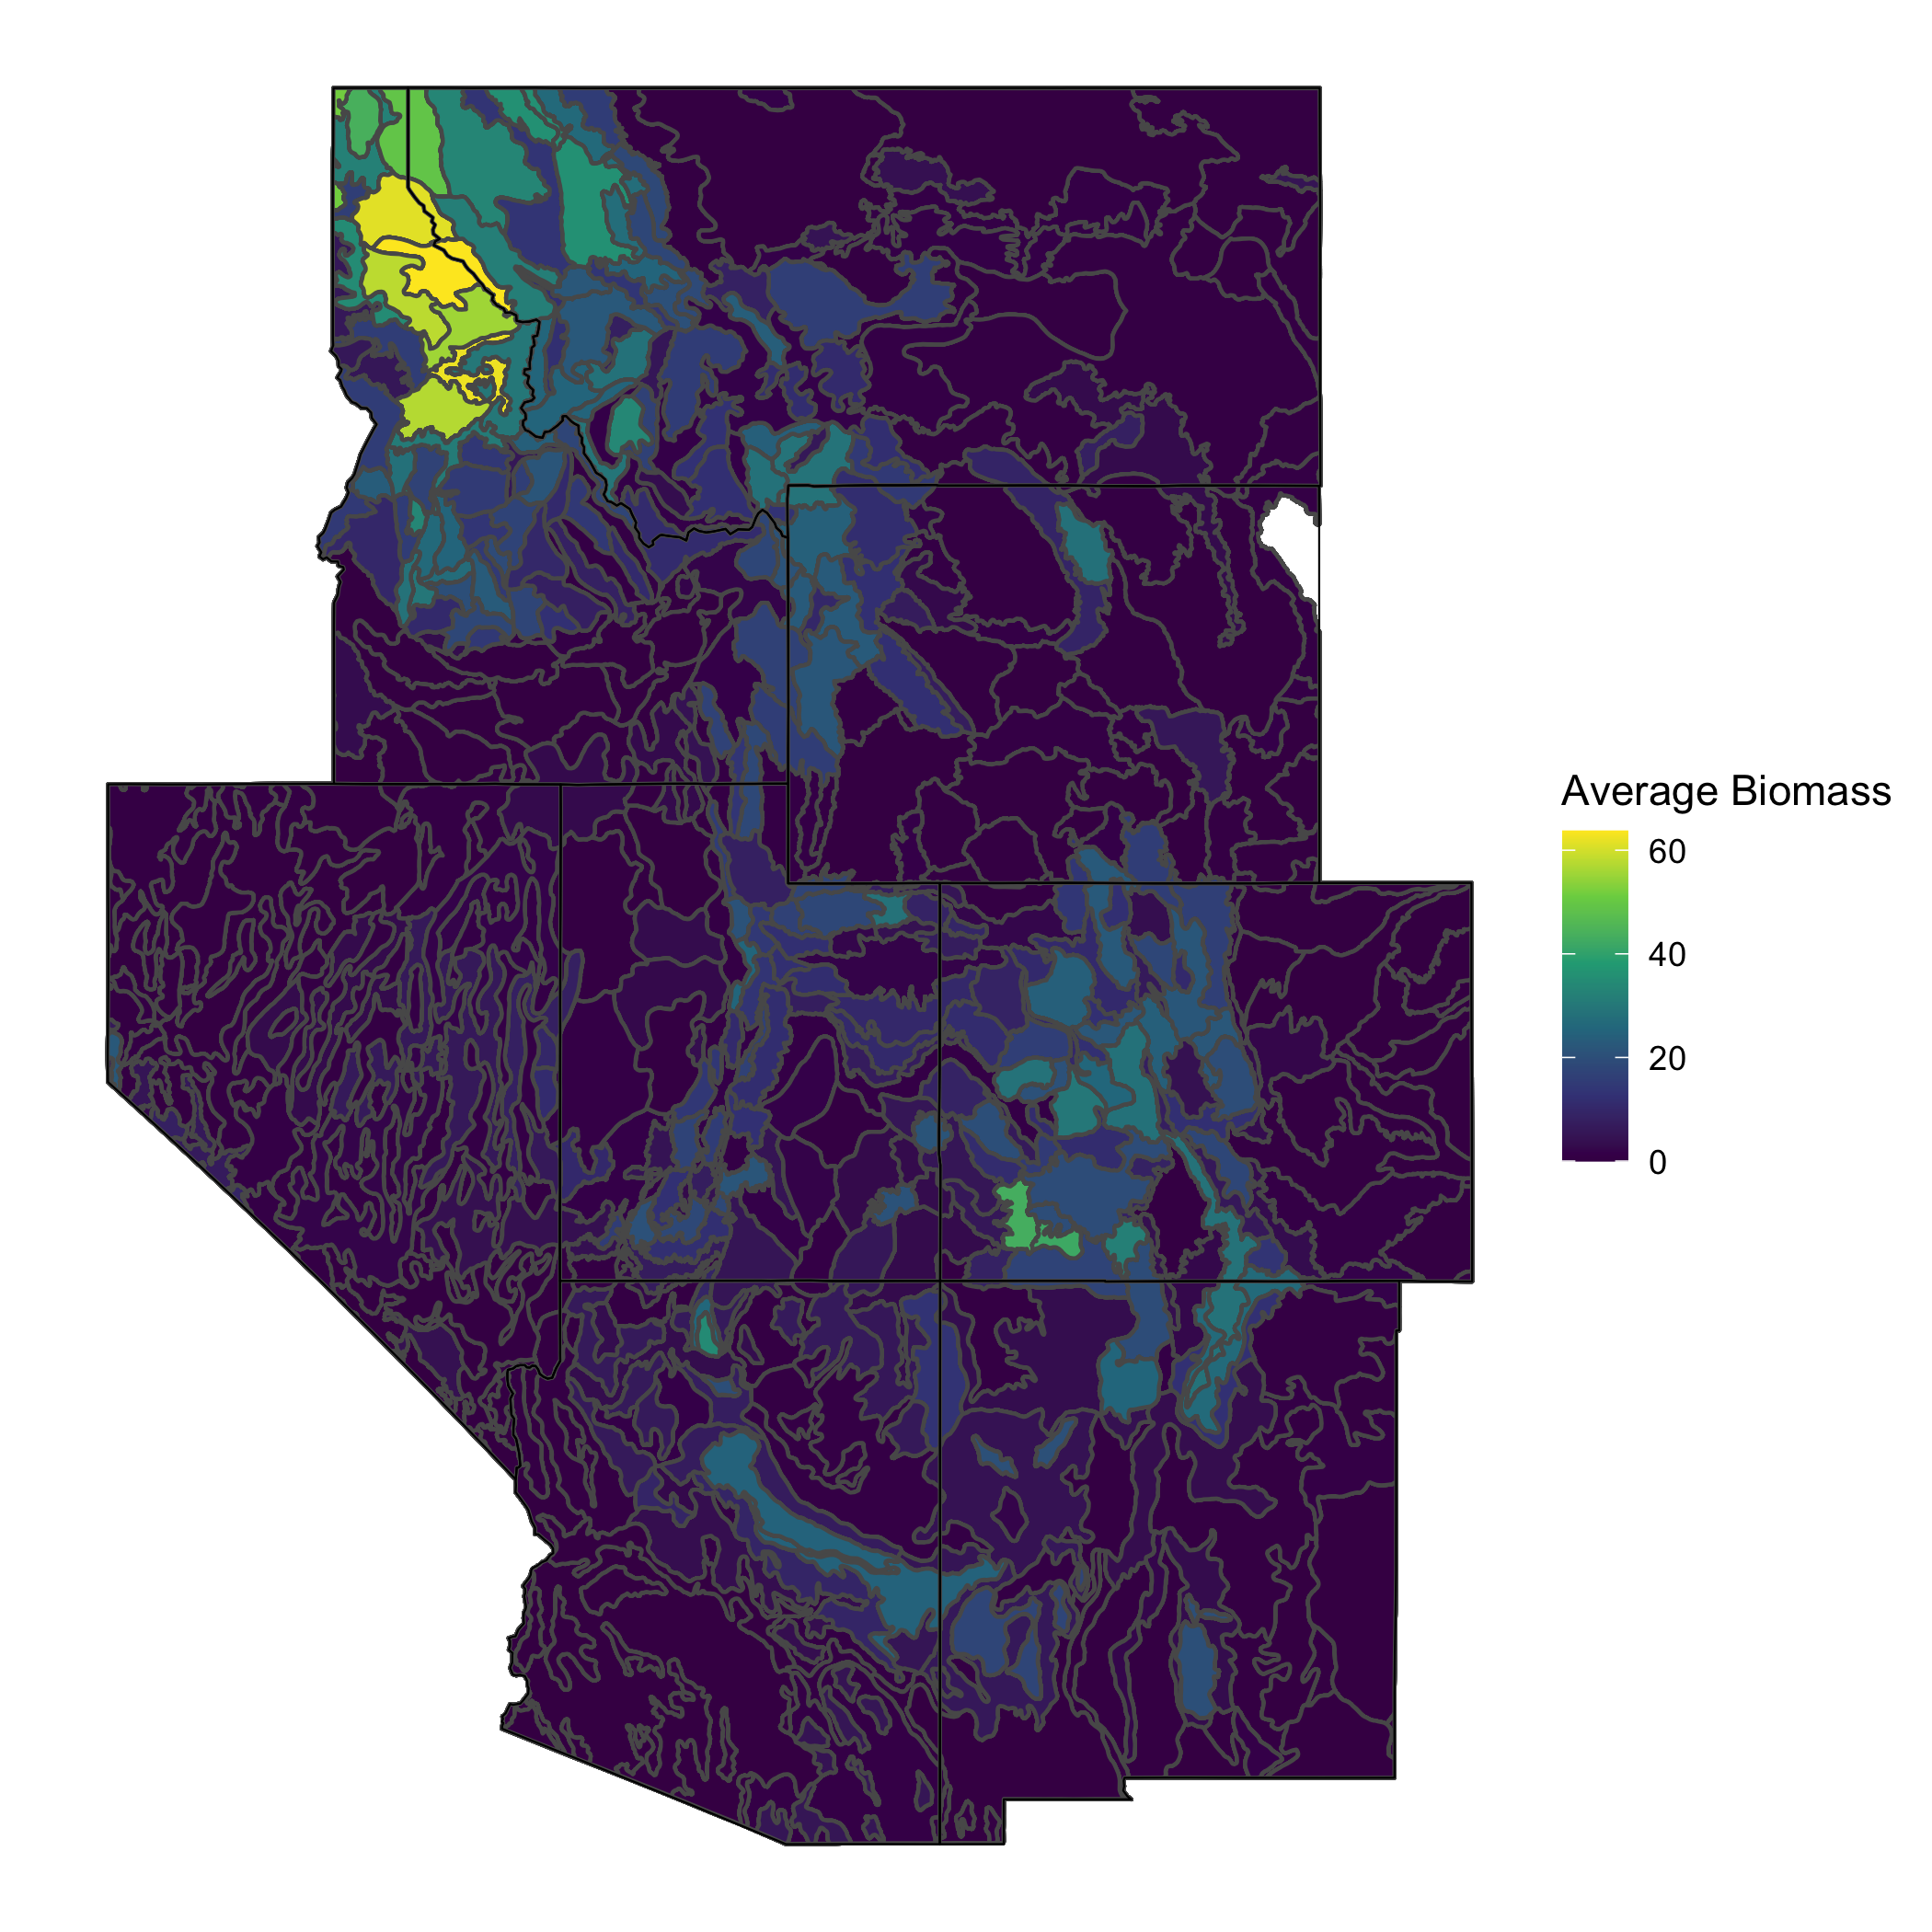
\includegraphics[width=0.65\linewidth,height=0.65\textheight]{figure/biomass} \end{center}
\begin{center}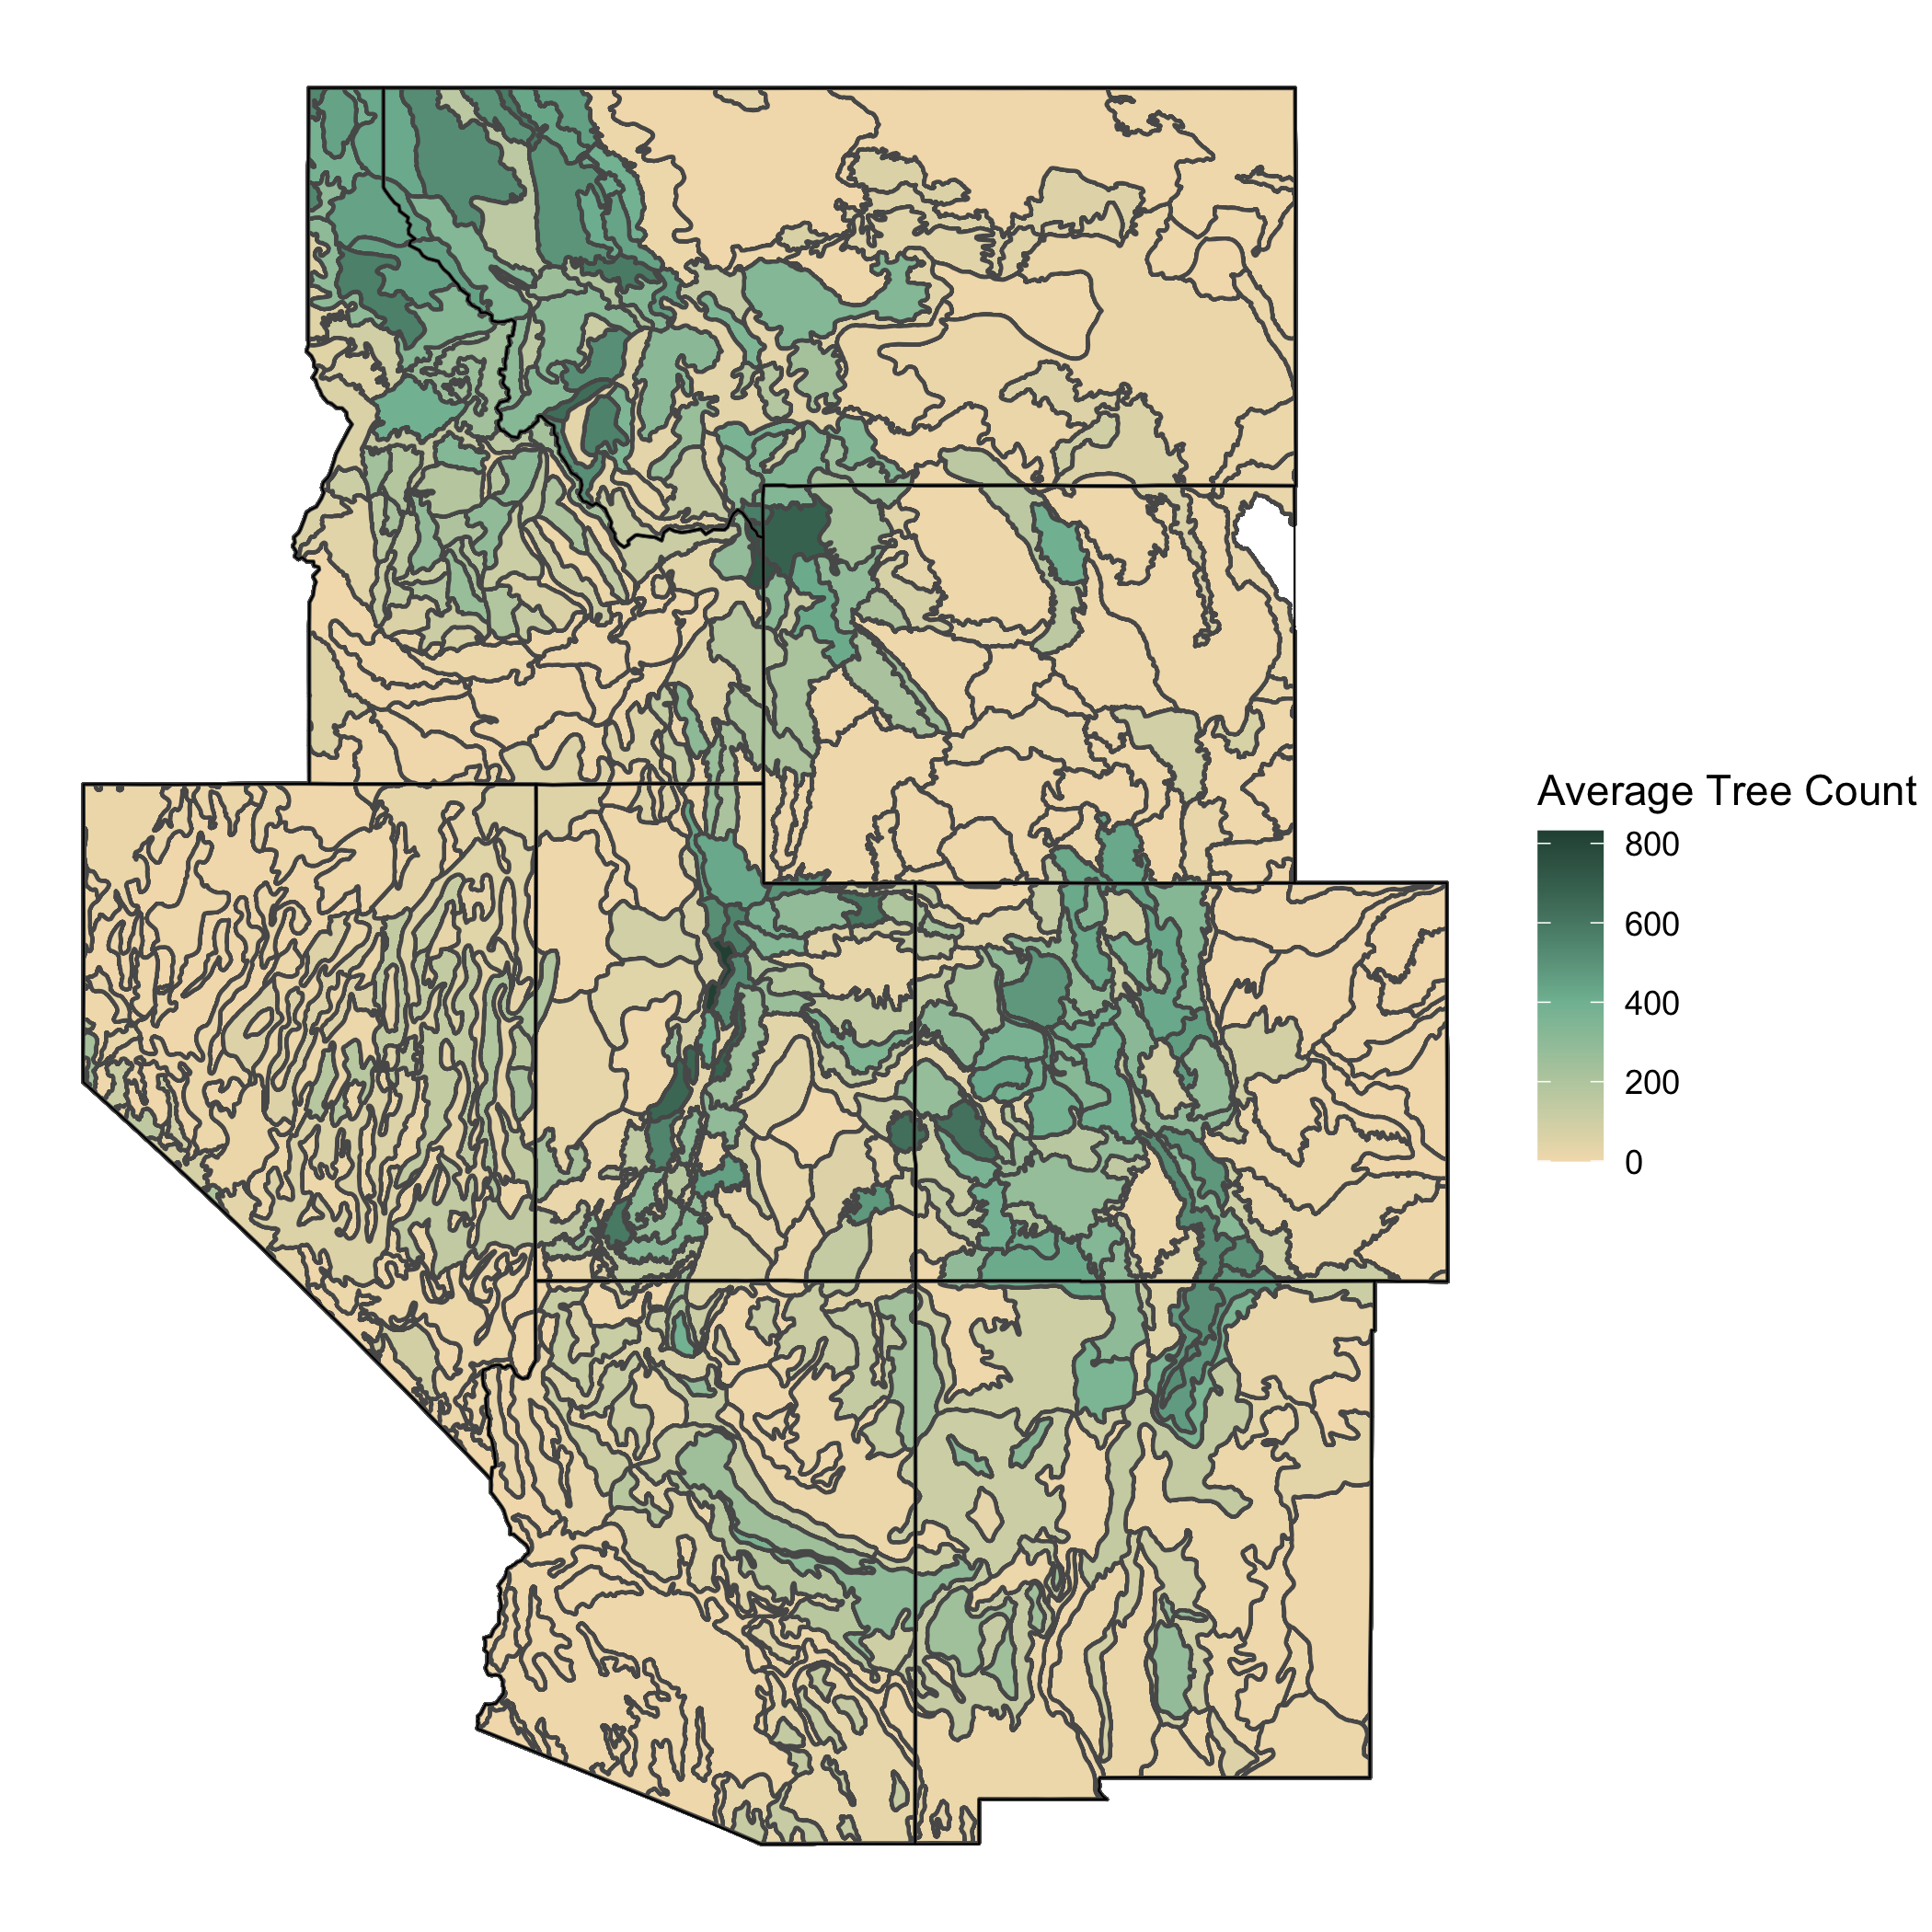
\includegraphics[width=0.65\linewidth,height=0.65\textheight]{figure/count} \end{center}
\begin{center}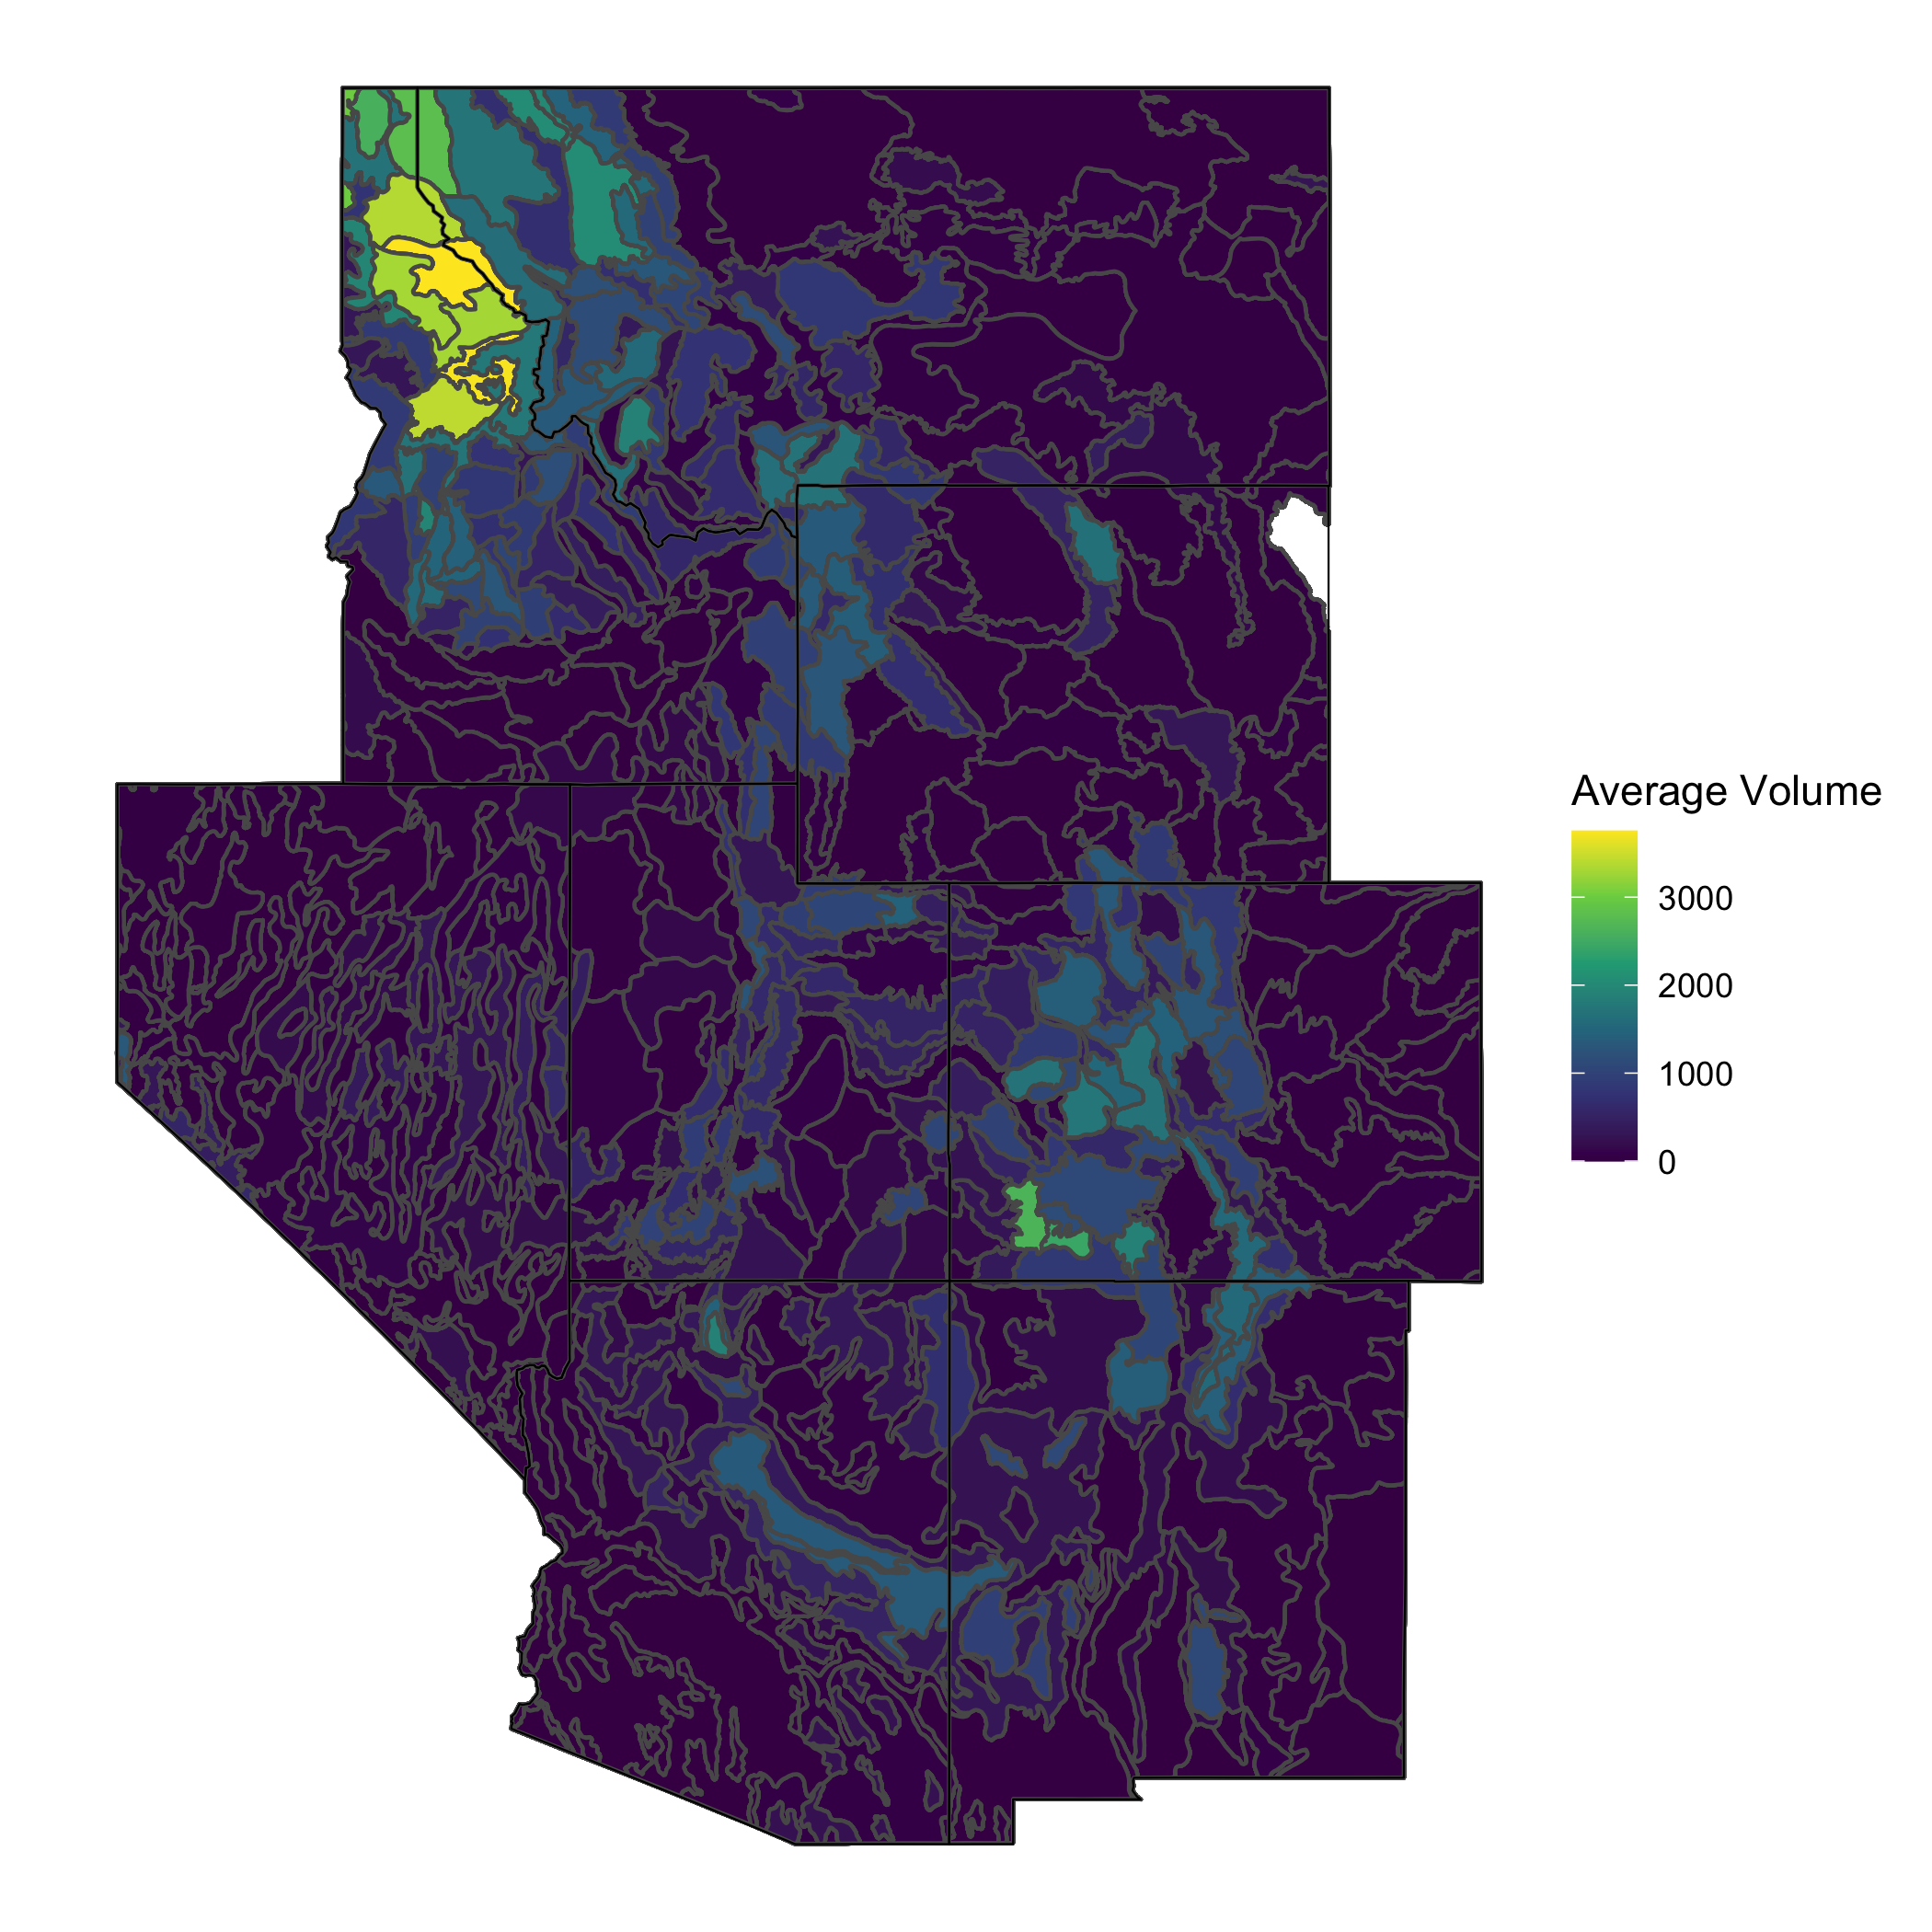
\includegraphics[width=0.65\linewidth,height=0.65\textheight]{figure/voln} \end{center}

While we have four variables which we will model as response variables throughout the analyses, we also have two predictor variables which will be of much use to us. In particular, forest probability and forest biomass (coded as \texttt{forprob} and \texttt{forbio}.) These variables which we will treat as predictors are remotely sensed variables, meaning that they were not collected by FIA crew members, but rather with aerial photography and/or satellite imagery. However, we will be using these variables to attempt to predict our response variables in order to understand how good of estimates we can make with this remote data that does not require as much effort to collect. While it may seem unnatural to attempt to predict forest biomass (\texttt{BIOLIVE\_TPA}) with forest biomass (\texttt{forbio}), the differences in the data collection process between the ground level data and remotely sensed data are quite different.

These variables are almost all right-skewed, and all take value zero quite often. To get a good sense of the distributions of the six key variables, we can look at histograms of each variable:
\begin{center}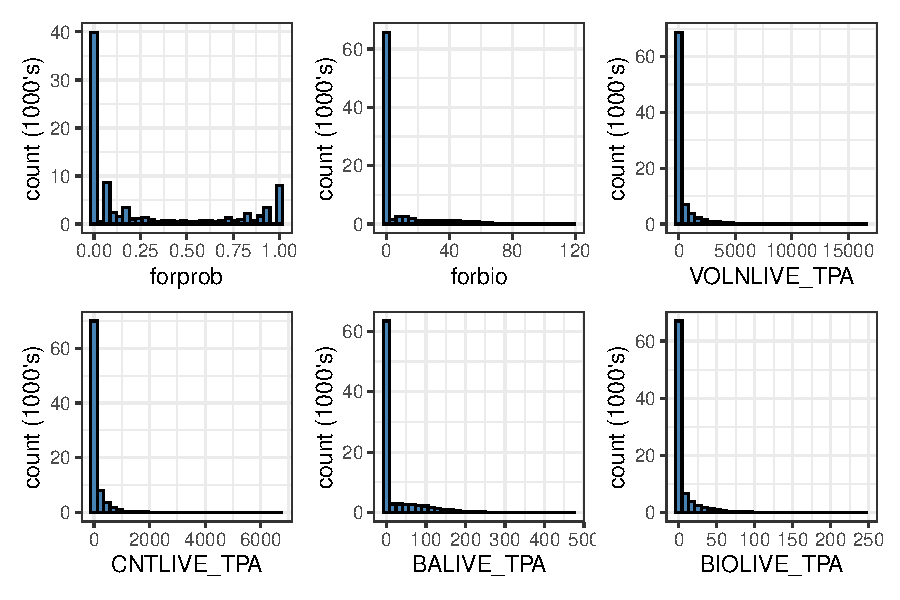
\includegraphics[width=432px]{thesis_files/figure-latex/unnamed-chunk-6-1} \end{center}

It is notable that the \texttt{forprob} variable is bimodal and modes zero and one, while all other variables are extremely right-skewed. This is likely because when \texttt{forprob} is decided from the remotely sensed data, there are likely areas that are either very clearly forest or very clearly not forest (residential areas, for example).

Apart from making histograms of our data, we can also summarize the data to see some summary statistics of our six key variables:

\captionsetup[table]{labelformat=empty,skip=1pt}
\begin{longtable}{lrrrrrrr}
\toprule
variable & mean & quantile\_25 & median & quantile\_75 & min & max & na\_count \\ 
\midrule
forbio & 6.66 & 0 & 0.00 & 0.00 & 0 & 118.00 & 0 \\ 
forprob & 0.27 & 0 & 0.07 & 0.56 & 0 & 1.00 & 1 \\ 
BIOLIVE\_TPA & 6.23 & 0 & 0.00 & 1.98 & 0 & 244.35 & 0 \\ 
BALIVE\_TPA & 22.75 & 0 & 0.00 & 14.75 & 0 & 469.39 & 0 \\ 
CNTLIVE\_TPA & 98.60 & 0 & 0.00 & 30.09 & 0 & 6677.93 & 0 \\ 
VOLNLIVE\_TPA & 342.32 & 0 & 0.00 & 74.69 & 0 & 16435.55 & 0 \\ 
\bottomrule
\end{longtable}
From this table, we can see how heavily skewed these key variables are, with over 25\% of the observations for each variable being zero. This does not stop us from doing meaningful analyses though, as the sample size of this dataset is so large (\(n = 86085\)) and thus we have plenty of data to create models with.

\hypertarget{data-structure-hierarchy}{%
\section{Data Structure \& Hierarchy}\label{data-structure-hierarchy}}

As hinted at throughout earlier parts of the chapter, the data used in this thesis has a hierarchical structure, where ecosubsections are nested within ecosections which are in turn nested within provinces. Every plot has each level of granularity of location data recorded and this is what allows us to choose how far to borrow strength from other plots.

The largest motivation for hierarchical modeling in this particular application is that observations are more similar within the hierarchies which we split them into. To understand if this is true, we can do a preliminary analysis on the data by performing three-way ANOVAs for each key variable with predictors \texttt{province}, \texttt{section}, and \texttt{subsection}. By just looking at the MSE of the ANOVA results, we can see that we should expect more homogeneity within ecosubsections:

\captionsetup[table]{labelformat=empty,skip=1pt}
\begin{longtable}{lrrr}
\toprule
variable & province\_MSE & ecosection\_MSE & ecosubsection\_MSE \\ 
\midrule
forbio & 614761.0 & 21713.4 & 6163.8 \\ 
forprob & 362.2 & 15.1 & 4.2 \\ 
BIOLIVE\_TPA & 500958.2 & 17910.5 & 5456.2 \\ 
BALIVE\_TPA & 3568986.3 & 118683.2 & 47835.7 \\ 
CNTLIVE\_TPA & 85365657.9 & 2512475.9 & 1287922.7 \\ 
VOLNLIVE\_TPA & 1559809302.3 & 60049667.7 & 18445636.8 \\ 
\bottomrule
\end{longtable}
(* Need a better way to output this table and show province level model is significant)

These results allow us to conclude that it is reasonable to believe that observations within a given province are more homogeneous than observations throughout the Interior West. Thus, if we want ecosubsection level estimates of variables, it makes sense to borrow information from other ecosubsections within the same province as each other. This data structure and homogeneity within provinces is what drives the analyses done henceforth in this thesis.

\hypertarget{conclusion}{%
\chapter*{Conclusion}\label{conclusion}}
\addcontentsline{toc}{chapter}{Conclusion}

If we don't want Conclusion to have a chapter number next to it, we can add the \texttt{\{-\}} attribute.

\textbf{More info}

And here's some other random info: the first paragraph after a chapter title or section head \emph{shouldn't be} indented, because indents are to tell the reader that you're starting a new paragraph. Since that's obvious after a chapter or section title, proper typesetting doesn't add an indent there.

\appendix

\hypertarget{the-first-appendix}{%
\chapter{The First Appendix}\label{the-first-appendix}}

This first appendix includes all of the R chunks of code that were hidden throughout the document (using the \texttt{include\ =\ FALSE} chunk tag) to help with readibility and/or setup.

\textbf{In the main Rmd file}
\begin{Shaded}
\begin{Highlighting}[]
\CommentTok{# This chunk ensures that the thesisdown package is}
\CommentTok{# installed and loaded. This thesisdown package includes}
\CommentTok{# the template files for the thesis.}
\ControlFlowTok{if}\NormalTok{ (}\OperatorTok{!}\KeywordTok{require}\NormalTok{(remotes)) \{}
  \ControlFlowTok{if}\NormalTok{ (params}\OperatorTok{$}\StringTok{`}\DataTypeTok{Install needed packages for \{thesisdown\}}\StringTok{`}\NormalTok{) \{}
    \KeywordTok{install.packages}\NormalTok{(}\StringTok{"remotes"}\NormalTok{, }\DataTypeTok{repos =} \StringTok{"https://cran.rstudio.com"}\NormalTok{)}
\NormalTok{  \} }\ControlFlowTok{else}\NormalTok{ \{}
    \KeywordTok{stop}\NormalTok{(}
      \KeywordTok{paste}\NormalTok{(}\StringTok{'You need to run install.packages("remotes")",}
\StringTok{            "first in the Console.'}\NormalTok{)}
\NormalTok{    )}
\NormalTok{  \}}
\NormalTok{\}}
\ControlFlowTok{if}\NormalTok{ (}\OperatorTok{!}\KeywordTok{require}\NormalTok{(thesisdown)) \{}
  \ControlFlowTok{if}\NormalTok{ (params}\OperatorTok{$}\StringTok{`}\DataTypeTok{Install needed packages for \{thesisdown\}}\StringTok{`}\NormalTok{) \{}
\NormalTok{    remotes}\OperatorTok{::}\KeywordTok{install_github}\NormalTok{(}\StringTok{"ismayc/thesisdown"}\NormalTok{)}
\NormalTok{  \} }\ControlFlowTok{else}\NormalTok{ \{}
    \KeywordTok{stop}\NormalTok{(}
      \KeywordTok{paste}\NormalTok{(}
        \StringTok{"You need to run"}\NormalTok{,}
        \StringTok{'remotes::install_github("ismayc/thesisdown")'}\NormalTok{,}
        \StringTok{"first in the Console."}
\NormalTok{      )}
\NormalTok{    )}
\NormalTok{  \}}
\NormalTok{\}}
\KeywordTok{library}\NormalTok{(thesisdown)}
\CommentTok{# Set how wide the R output will go}
\KeywordTok{options}\NormalTok{(}\DataTypeTok{width =} \DecValTok{70}\NormalTok{)}
\end{Highlighting}
\end{Shaded}
\textbf{In Chapter \ref{ref-labels}:}

\hypertarget{the-second-appendix-for-fun}{%
\chapter{The Second Appendix, for Fun}\label{the-second-appendix-for-fun}}

\backmatter

\hypertarget{references}{%
\chapter*{References}\label{references}}
\addcontentsline{toc}{chapter}{References}

\markboth{References}{References}

\noindent

\setlength{\parindent}{-0.20in}
\setlength{\leftskip}{0.20in}
\setlength{\parskip}{8pt}

\hypertarget{refs}{}
\leavevmode\hypertarget{ref-angel2000}{}%
Angel, E. (2000). \emph{Interactive computer graphics : A top-down approach with opengl}. Boston, MA: Addison Wesley Longman.

\leavevmode\hypertarget{ref-angel2001}{}%
Angel, E. (2001a). \emph{Batch-file computer graphics : A bottom-up approach with quicktime}. Boston, MA: Wesley Addison Longman.

\leavevmode\hypertarget{ref-angel2002a}{}%
Angel, E. (2001b). \emph{Test second book by angel}. Boston, MA: Wesley Addison Longman.


% Index?

\end{document}
